\documentclass[a4paper,10pt,twocolumn]{article}

\usepackage[T1]{fontenc}
\usepackage[utf8]{inputenc}
\usepackage{microtype}
\usepackage[margin=18mm,top=19mm,bottom=21mm,columnsep=7mm]{geometry}
\usepackage{amsmath}
\usepackage{graphicx}
\usepackage{booktabs}
\usepackage{tabularx}
\usepackage{array}
\usepackage{float}
\usepackage{balance}
\usepackage{enumitem}
\usepackage[numbers,sort&compress]{natbib}
\usepackage{xcolor}
\usepackage{url}
\usepackage[hidelinks]{hyperref}

\graphicspath{{../figures/}}
\setlength{\emergencystretch}{1.5em}
\setlist{nosep,leftmargin=*}
\raggedbottom

\newcommand{\rf}{\ensuremath{\mathrm{RF}}}
\newcommand{\cockroach}{CockroachDB}
\newcommand{\hdfs}{HDFS}
\newcommand{\qps}{QPS}
\newcommand{\todoauthor}{Anonymous Author(s)}
\newcommand{\todoaffiliation}{Affiliation omitted in working draft}

\title{\textbf{When More Replicas Do Not Help:}\\
Testing File-Storage Replication Intuition in Distributed SQL}
\author{\todoauthor\\\small \todoaffiliation}
\date{}

\begin{document}

\maketitle

\begin{abstract}
Replication-factor adaptation is well motivated in distributed file storage,
where an additional block copy may improve locality, distribute concurrent
reads, or protect another failure domain. This paper investigates whether the
same tuning intuition transfers to a consensus-based distributed SQL database.
\cockroach{} is the primary object of study; \hdfs{} is used as an
architectural and experimental contrast that exposes why replication can act
as a read-scaling mechanism in file storage. In \cockroach{}, replicas
participate in Raft groups, transactions, and leaseholder-directed execution,
so an additional voting replica does not automatically create an independent
path for strongly consistent reads. Rather than proposing a new adaptation
algorithm, we first test whether \rf{} is an effective and predictable
database control action. A validated local \cockroach{} ladder covering
\rf{} 3, 5, and 7 completed all 27 runs without workload or collection errors.
Read-only and most 80:20 runs reached a configured 150 \qps{} cap, while the
saturated 50:50 series was variable and non-monotonic. A smaller \hdfs{}
contrast showed that reader parallelism, rather than \rf{}, dominated local
throughput. These preliminary results do not justify generic database
\rf{} adaptation. They instead identify the conditions under which it may be
useful: failure-domain requirements, deliberate leaseholder placement,
eligible follower reads, geographic locality, and a workload stable enough to
amortize reconfiguration.
\end{abstract}

\noindent\textbf{Keywords:} replication factor, distributed SQL, CockroachDB,
HDFS, Raft, distributed storage, performance evaluation

\section{Introduction}
\label{sec:introduction}

Replication level and replica placement are established control mechanisms in
distributed file systems. The Google File System (GFS) stores chunks across
commodity machines to provide fault tolerance and high aggregate
performance~\citep{ghemawat2003gfs}. \hdfs{} similarly exposes a configurable
per-file replication factor and combines rack-aware placement with
nearest-replica selection~\citep{shvachko2010hdfs}. Later systems made
replication explicitly workload-aware. Scarlett creates additional replicas
for popular content in MapReduce clusters~\citep{ananthanarayanan2011scarlett},
while Copyset Replication shows that the placement pattern of a fixed number of
replicas can materially change durability under correlated
failures~\citep{cidon2013copysets}. This work creates a plausible systems
intuition: if demand becomes read-heavy or geographically skewed, create more
replicas near that demand.

This paper asks whether that intuition transfers to a distributed SQL
database. In a file system, another block replica can become another physical
read source. In a database such as \cockroach{}, another voting replica joins
a consistency and transaction protocol. Raft orders replicated state-machine
updates through a leader and commits log entries after majority
agreement~\citep{ongaro2014raft}. \cockroach{} applies this model to key ranges
and combines it with leases and distributed transaction
processing~\citep{taft2020cockroach}. Increasing \rf{} therefore changes
failure tolerance, replication fan-out, majority size, and placement choices,
but it does not automatically create another independent path for strongly
consistent reads.

\cockroach{} is the research target, while \hdfs{} provides the contrast. The
\hdfs{} experiment is not a product benchmark. It illustrates the mechanism
from which \rf{} tuning intuition originates and provides a reference for
interpreting database behavior. We intentionally stop before algorithm design:
an adaptive controller is useful only if changing \rf{} produces a repeatable
benefit, the workload remains in that regime long enough to amortize
reconfiguration, and the controller can observe the mechanism causing the
benefit.

This paper makes three contributions:

\begin{enumerate}
  \item It evaluates \rf{} as a performance-control action in a
  consensus-based distributed SQL database.
  \item It uses file storage to explain why another replica can improve reads
  in one architecture but does not automatically do so in a database.
  \item It provides a reproducible experimental scaffold and a
  mechanism-based decision framework for future database \rf{} adaptation.
\end{enumerate}

The evidence is preliminary and local. The contribution is therefore not a
claim that one \rf{} is universally optimal. It is a narrower result: the
present measurements do not show a stable monotonic performance benefit from
increasing \cockroach{} \rf{}, and the architecture explains why such a
benefit requires additional conditions.

\section{Background and Prior Work}
\label{sec:background}

\subsection{Replication in file storage}

\hdfs{} separates metadata coordination from the data path. The NameNode
manages the namespace, block locations, replication decisions, and placement
policy. DataNodes store blocks and serve client reads and writes. After
obtaining block locations, clients transfer data directly to or from a
DataNode~\citep{shvachko2010hdfs}. Another replica can therefore become a
closer read source, distribute concurrent demand, or cover an additional
failure domain.

These benefits remain conditional. They depend on physical placement,
topology, cache state, scheduling, and sufficient concurrent demand. Higher
\rf{} also consumes storage, sends more replication traffic, expands the write
pipeline, and creates background work when the setting changes. Scarlett
demonstrates the positive case: long-lived content popularity can justify
selective block replication because the new copies relieve real storage-node
hotspots~\citep{ananthanarayanan2011scarlett}.

\subsection{Consensus-based distributed SQL}

Raft manages a replicated log and tolerates failures by committing entries
after a majority of voters acknowledges them~\citep{ongaro2014raft}. For
\(n\) voters, a majority contains
\(\lfloor n/2 \rfloor + 1\) replicas. Increasing \rf{} changes both the
replication fan-out and, at some transitions, the majority size. This is not
the passive-copy model implied by file storage.

\cockroach{} partitions data into ranges, each represented by a Raft
replication group~\citep{taft2020cockroach}. A Raft leader orders log entries,
while a range leaseholder coordinates most strong reads and proposes writes.
The leader and leaseholder are related operational roles but should not be
conflated conceptually. In particular, a strong read does not consult a quorum
for every request, yet arbitrary voting replicas do not become generic strong
read servers: requests are normally routed through the leaseholder. Follower
reads can use non-leaseholder replicas, including geographically close ones,
but they introduce a different freshness contract.

Geo-distributed databases also demonstrate that replica count cannot be
separated from placement and consistency. Spanner combines synchronous
replication with explicit geographic configuration and globally meaningful
time~\citep{corbett2012spanner}. Its design illustrates both sides of the
trade-off: replicas can place data near users and survive regional failures,
while a geographically distributed write quorum can put wide-area delay on
the commit path. More generally, classical work warns that replication can
create substantial coordination cost when updates must remain
consistent~\citep{gray1996dangers}.

\subsection{Positioning}

Prior file-storage work asks how to place or add copies once replicas are known
to be useful read-serving objects. Prior database work explains consensus,
transactions, and geo-distribution. This paper connects the two by asking a
step that precedes controller design: is changing the number of database
replicas itself a useful and predictable performance action? The \hdfs{}
experiment is included only to expose the architectural source of the
file-storage intuition.

\section{Research Questions}
\label{sec:questions}

The study is organized around three research questions:

\begin{enumerate}[label=\textbf{RQ\arabic*.},leftmargin=*]
  \item Does increasing \rf{} improve \cockroach{} throughput
  or latency under strong read-only and mixed read/write workloads?
  \item Do the database results exhibit the read-scaling
  behavior that motivates \rf{} adaptation in file storage?
  \item Under which consistency, placement, workload-duration,
  and geographic conditions could \rf{} adaptation still be worthwhile in
  distributed SQL?
\end{enumerate}

Table~\ref{tab:architecture} summarizes the mechanism-level contrast. The
important distinction is not that file systems always benefit from higher
\rf{}. It is that another file block copy is directly eligible to serve reads,
whereas another database voter is primarily part of a replicated state
machine.

\begin{table*}[t]
\centering
\caption{The same replication-factor parameter activates different mechanisms
in file storage and consensus-based distributed SQL.}
\label{tab:architecture}
\small
\begin{tabularx}{\textwidth}{@{}>{\raggedright\arraybackslash\bfseries}p{0.18\textwidth}
                              X
                              X@{}}
\toprule
Tuning question & File-storage intuition & Distributed SQL implication \\
\midrule
Can another replica serve reads?
  & Normally yes, subject to placement and client selection.
  & Not for arbitrary strong reads; leaseholder or follower-read rules apply. \\
What does \rf{} primarily change?
  & Number and location of physical block copies.
  & Consensus membership, failure tolerance, placement, and replication fan-out. \\
Where can read performance improve?
  & Locality, parallel service, and storage-node load distribution.
  & Leaseholder placement or eligible local follower reads. \\
What is the main incremental cost?
  & Storage, write pipeline, transfer, and re-replication.
  & Storage, write replication, majority coordination, and range rebalancing. \\
\bottomrule
\end{tabularx}
\end{table*}

\section{Experimental Methodology}
\label{sec:method}

\subsection{Primary database experiment}

The local \cockroach{} deployment contains nine Docker containers on one
Windows host. A synthetic benchmark table contains 90,000 rows and is
configured as one range to make the tested replication group explicit. The
table is recreated before each run. The workload generator addresses all nine
nodes with two workers per node and uses strong reads.

The validated safe ladder varies:

\begin{itemize}
  \item \rf{} values 3, 5, and 7;
  \item read/write ratios 100:0, 80:20, and 50:50;
  \item three repetitions per configuration;
  \item 90 seconds of measured workload and 30 seconds of cooldown; and
  \item a total target rate of 150 \qps{}.
\end{itemize}

The 27 configurations are shuffled to reduce monotonic-order bias from thermal
effects, background compaction, and replica movement. Each run records actual
\qps{}, successful and failed operations, connection errors, and collection
errors. The result directory is accepted only if the full
\rf{}-ratio-repetition matrix exists, all workload error counts are zero, load
files are readable, metrics contain no error rows, and all nine containers
remain running.

The ladder used a legacy native-metrics collector that stored already-computed
cumulative p90 and p99 snapshots from one node. Such values combine activity
from before the workload and are not cluster-wide per-run latency. They are
preserved as diagnostic data but excluded from the paper. The corrected
collector records raw cumulative histogram buckets and counters from all
nodes, then computes end-minus-start deltas over the workload interval. A
repeat run is required before native SQL/KV latency can be reported.

The 150 \qps{} cap is also important. A run that reaches the target proves that
the configuration sustains the selected load; it does not estimate maximum
capacity. Conversely, low achieved \qps{} is reported as saturation rather
than silently treating target throughput as controlled.

\subsection{File-storage contrast}

The \hdfs{} deployment contains one NameNode, five DataNodes, and one client
container on the same physical host. The seed sweep varies \rf{} from 1 to 5,
uses four synthetic 64 MiB files, and measures 1, 2, 4, and 8 parallel readers.
Every combination is repeated twice in randomized order. For each \rf{}, the
benchmark writes the data set, waits for \texttt{hdfs dfs -setrep -w} to
complete, and then measures aggregate read throughput.

The \hdfs{} data are accepted only if the complete
\rf{}-reader-repetition matrix exists and all write and read measurements are
positive. This experiment is deliberately smaller than the database ladder.
Its role is to show the distinct read-serving mechanism, not to rank two
different products.

\subsection{Analysis and evidence classes}

The repository distinguishes smoke tests, preliminary local evidence, and
paper-grade evidence. This paper reports validated preliminary evidence. Means
and sample standard deviations are computed across repetitions, but the small
sample sizes do not justify formal significance tests. Raw result directories
retain metadata, command parameters, logs, and per-run outputs. Compact
per-run and grouped CSV summaries are curated with the paper.

The failed local \cockroach{} \rf{}=9 attempt is excluded from performance
curves. It destabilized the nine-container setup and is retained only as
evidence of an environment limit.

\section{Results}
\label{sec:results}

\subsection{\cockroach{} target attainment}

All 27 planned runs completed with zero connection, read, write, or metrics
errors. Table~\ref{tab:cockroach-qps} reports actual \qps{} as mean and sample
standard deviation across three repetitions.

\begin{table}[H]
\centering
\caption{\cockroach{} actual \qps{}, mean (standard deviation), \(n=3\).}
\label{tab:cockroach-qps}
\small
\setlength{\tabcolsep}{3pt}
\begin{tabular}{@{}lrrr@{}}
\toprule
Read:write & \rf{}=3 & \rf{}=5 & \rf{}=7 \\
\midrule
100:0 & 149.71 (0.30) & 149.71 (0.27) & 149.47 (0.67) \\
80:20 & 149.37 (0.57) & 149.80 (0.16) & 145.24 (6.00) \\
50:50 & 133.20 (6.84) & 138.50 (13.33) & 129.86 (16.14) \\
\bottomrule
\end{tabular}
\end{table}

\begin{figure}[H]
\centering
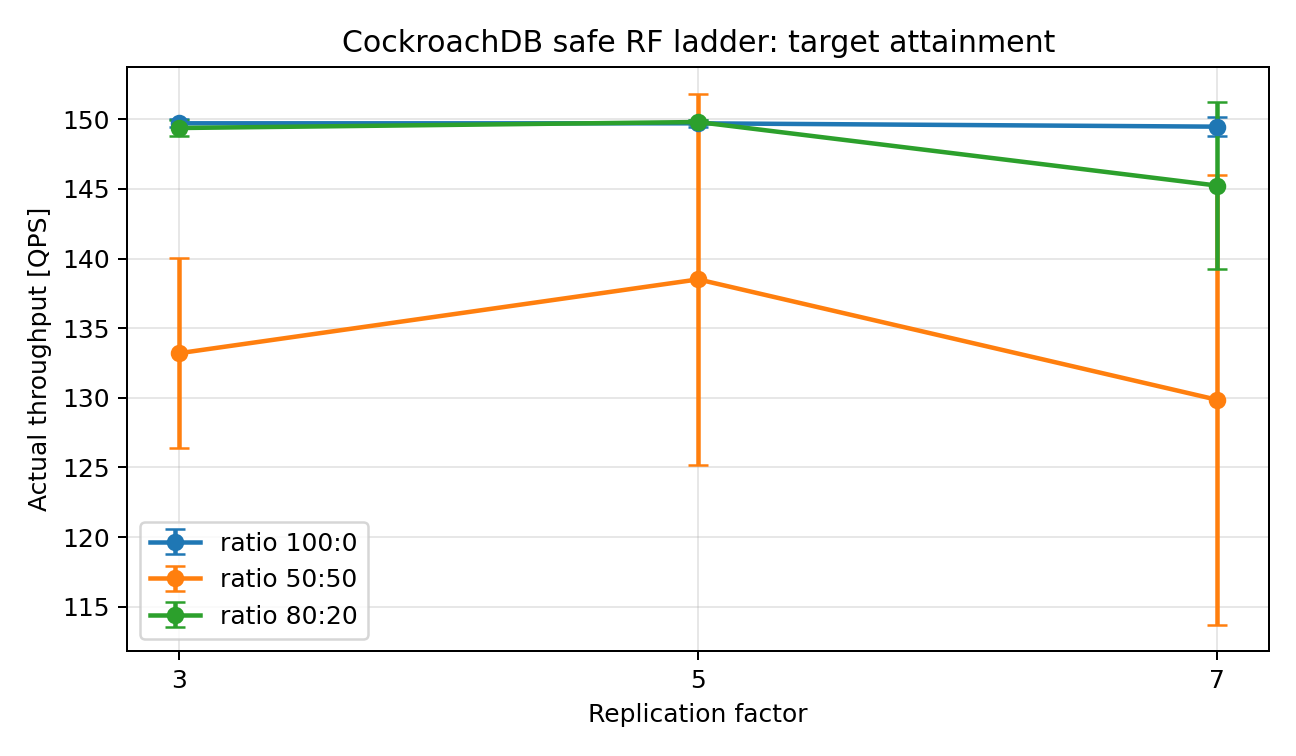
\includegraphics[width=\columnwidth]{preliminary_cockroach_safe_rf_ladder.png}
\caption{\cockroach{} target attainment. Error bars show one sample standard
deviation. The 150 \qps{} target caps read-only and most 80:20 observations.}
\label{fig:cockroach}
\end{figure}

The read-only workload reaches the 150 \qps{} target at every \rf{} with very
little variation. This demonstrates stability at the selected load, but cannot
establish equal maximum capacity or a read-scaling benefit. \rf{}=3 and
\rf{}=5 similarly reach the target in the 80:20 workload, while \rf{}=7
averages 145.24 \qps{} and varies more strongly.

The 50:50 workload exposes a clearer saturation regime. Mean throughput is
non-monotonic and variation is substantial. \rf{}=5 has the highest mean, but
its standard deviation is nearly twice that of \rf{}=3. \rf{}=7 has both the
lowest mean and the largest spread. No increasing \rf{} sequence provides a
stable monotonic improvement.

The result is consistent with the architectural expectation: voting replicas
do not act as independent strong-read servers and can interact with consensus
work, leaseholder placement, range reconfiguration, and shared-host
contention. It does not prove that \rf{}=3 is optimal; the capped and small
experiment cannot support that claim.

\subsection{\hdfs{} contrast}

The \hdfs{} seed completed all 40 planned measurements and passed validation.
Table~\ref{tab:hdfs} reports mean read throughput across two repetitions.

\begin{table}[H]
\centering
\caption{\hdfs{} mean read throughput in MiB/s, \(n=2\).}
\label{tab:hdfs}
\small
\begin{tabular}{@{}rrrrr@{}}
\toprule
\rf{} & 1 reader & 2 readers & 4 readers & 8 readers \\
\midrule
1 & 14.67 & 26.13 & 40.69 & 49.73 \\
2 & 15.87 & 25.05 & 38.59 & 43.92 \\
3 & 16.56 & 27.86 & 40.06 & 48.82 \\
4 & 17.48 & 27.24 & 40.46 & 53.24 \\
5 & 16.21 & 26.01 & 39.87 & 50.12 \\
\bottomrule
\end{tabular}
\end{table}

\begin{figure}[H]
\centering
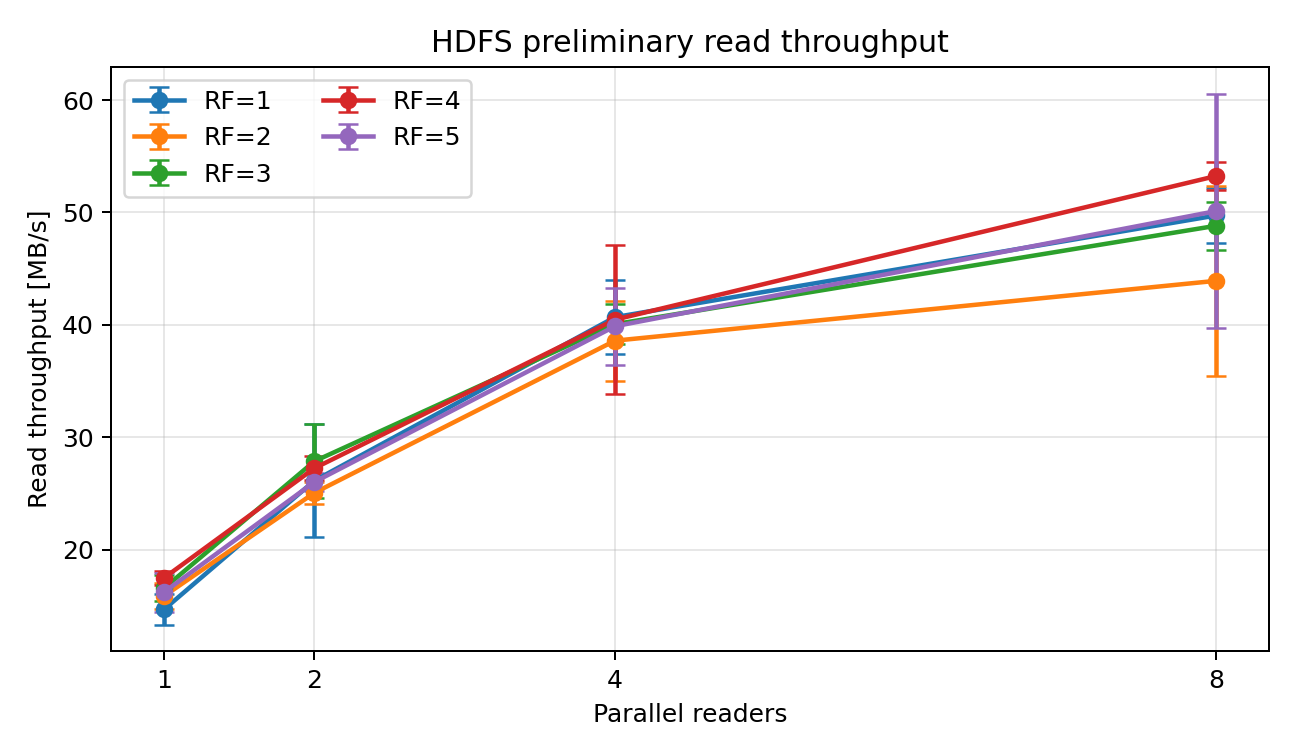
\includegraphics[width=\columnwidth]{preliminary_hdfs_read_throughput.png}
\caption{\hdfs{} read throughput. Reader parallelism dominates the local
result; \rf{} remains smaller and non-monotonic. Error bars show one sample
standard deviation.}
\label{fig:hdfs}
\end{figure}

The clearest pattern is scaling with reader count, not with \rf{}. Moving from
one to eight readers increases throughput by roughly three times across all
\rf{} settings. The \rf{} effect is smaller and non-monotonic: \rf{}=4 is best
for one and eight readers, while \rf{}=3 is best for two readers and \rf{}=1
is close to the best result for four readers.

This does not establish that increasing \rf{} always improves \hdfs{}
performance. It establishes the narrower architectural contrast: another
block copy is eligible to serve a nearby or concurrent reader, even though the
shared-host experiment does not isolate locality or storage-node load
distribution. Strong \cockroach{} reads lack a corresponding generic path.

\subsection{Answers to the research questions}

\textbf{RQ1.} The preliminary ladder provides no
evidence of a stable monotonic \cockroach{} throughput benefit as \rf{}
increases. Capped runs establish target attainment only, while saturated 50:50
runs are non-monotonic and variable. Valid latency results remain pending.

\textbf{RQ2.} The file-storage intuition does not
transfer directly. File replicas are potential read sources; database voters
are consensus participants. The current \hdfs{} data do not show a monotonic
\rf{} benefit either, but they expose a different read-serving mechanism.

\textbf{RQ3.} Database \rf{} adaptation is
plausible only when it activates a concrete benefit: required failure-domain
coverage, improved leaseholder placement, eligible follower reads, useful
geographic locality, or a persistent workload that can amortize range
replication and rebalancing.

\section{Implications for RF Tuning}
\label{sec:discussion}

\subsection{Resilience is the default benefit}

The most direct reason to increase \cockroach{} \rf{} is a required
failure-tolerance level. More voters can cover additional node, zone, or region
failures. Replica count alone is insufficient, however: Copysets illustrates
that the correlation structure of placement can matter as much as the nominal
number of copies~\citep{cidon2013copysets}. An operator should therefore state
the decision as a failure-domain and placement requirement, not merely as a
larger integer.

\subsection{Eligible read paths}

The file-storage contrast exposes the missing mechanism. In \hdfs{}, the
client can select a nearby block replica and concurrent readers can distribute
work over DataNodes. \cockroach{} obtains an analogous locality benefit only
when reads are eligible to use the added replica. This can occur through
deliberate leaseholder placement or follower reads with acceptable staleness.
Without such a path, increasing \rf{} for a read-heavy strong-consistency
workload has no clear reason to increase read-serving capacity.

\subsection{Geographic benefits and costs}

Geography can make a database replica valuable when placement converts remote
access into local access. It also makes coordination more expensive. A remote
voter may improve regional survivability while putting wide-area latency on
the write quorum. A nearby replica improves foreground reads only when the
leaseholder is placed appropriately or the application accepts follower-read
freshness. Strong leaseholder reads, bounded-staleness follower reads, and
geographically distributed writes must therefore be evaluated separately.

\subsection{Amortizing reconfiguration}

Dynamic \rf{} changes create replicas, move range data, and trigger
rebalancing. A controller reacting to a short burst may finish only after the
burst disappears. Reconfiguration can also overlap with lease transfers,
range movement, compaction, and background maintenance. A useful policy must
estimate both the magnitude and the duration of the expected benefit.

Conceptually, increasing database \rf{} is defensible only when

\begin{equation}
\label{eq:decision}
\begin{aligned}
B_{\mathrm{resilience}} + B_{\mathrm{locality}}
> {} & C_{\mathrm{storage}} + C_{\mathrm{write}} \\
     & + C_{\mathrm{migration}} + C_{\mathrm{coordination}} .
\end{aligned}
\end{equation}

The terms need not use one monetary unit in an implementation, but the
inequality forces the policy to name the active benefit. ``Read-heavy'' alone
is not enough.

\subsection{Next evidence needed}

A paper-grade database evaluation should:

\begin{enumerate}
  \item use at least 180-second randomized runs with at least three, preferably
  five, repetitions;
  \item sweep offered load to locate capacity boundaries instead of capping
  all read-heavy cases at one target;
  \item report client p50/p90/p99 latency and cluster-wide native SQL/KV
  p90/p99 from per-run histogram deltas;
  \item compare strong reads with a separately labeled follower-read series;
  and
  \item use a multi-host or controlled-network setup for geographic claims.
\end{enumerate}

\section{Threats to Validity}
\label{sec:threats}

\textbf{Shared host.} All logical nodes share one physical CPU, memory system,
disk subsystem, and network stack. Docker Desktop and the host scheduler can
produce contention that would differ on independent machines. The setup cannot
demonstrate rack or regional locality.

\textbf{Workload scope.} The \cockroach{} workload uses one synthetic table,
one range, controlled operation mixes, and uniform target rates. Real
applications may include multiple ranges, secondary indexes, multi-statement
transactions, skew, and application-level think time.

\textbf{Target-rate censoring.} Read-only and most 80:20 runs reach the 150
\qps{} cap. They show successful target attainment, not maximum throughput.
Only the lower achieved rates provide saturation evidence.

\textbf{Latency instrumentation.} Native latency snapshots from the safe ladder
are cumulative and single-node. Excluding them avoids a false per-run claim,
but leaves RQ1 only partially answered until the corrected collector is used.

\textbf{Reconfiguration effects.} Changing \rf{} can cause replica movement,
lease transfer, compaction, and other background activity. Cooldown and
randomization reduce but do not remove these effects.

\textbf{File-storage contrast.} The \hdfs{} seed uses two repetitions,
synthetic zero-filled files, and one shared host. It does not prove that higher
\rf{} generally improves file-system reads. It only demonstrates the
architectural availability of multiple block sources.

\textbf{External validity.} Conclusions concern this \cockroach{} version,
configuration, strong-read mode, and local environment. They should not be
generalized to all distributed SQL systems or all replica types.

\section{Conclusion}
\label{sec:conclusion}

This paper studies replication-factor tuning in distributed SQL by testing an
intuition inherited from file storage. In a file system, another block replica
may become another read source. In \cockroach{}, another voting replica
primarily changes fault tolerance, placement, and replicated state-machine
topology. It improves read performance only when leaseholder placement or
follower-read behavior makes the replica eligible to serve useful demand.

The validated preliminary ladder completed without errors but showed no stable
monotonic throughput improvement as \rf{} increased from 3 to 7. Read-heavy
runs were capped by the offered load, and the saturated 50:50 series was
variable and non-monotonic. These results do not justify a new generic
database \rf{} adaptation algorithm. They support a more careful rule: change
\rf{} only when a named benefit---failure-domain coverage, leaseholder
placement, eligible local follower reads, or consistency-aware geographic
placement---can plausibly exceed storage, write, coordination, and
reconfiguration costs.

\section*{Artifact Availability}

The experiment runners, validation scripts, curated preliminary CSV files, and
figure-generation code are available at
\url{https://github.com/janraj00/replication-factor-study}. Raw generated
result directories remain separate from the repository; compact summaries and
metadata document the evidence used here.

\setlength{\bibsep}{2pt}
\balance
\bibliographystyle{plainnat}
\bibliography{references}

\end{document}
